\section{Konzept}

\subsection{Kontextdiagramm}
\begin{figure}[H]
  \begin{center}
    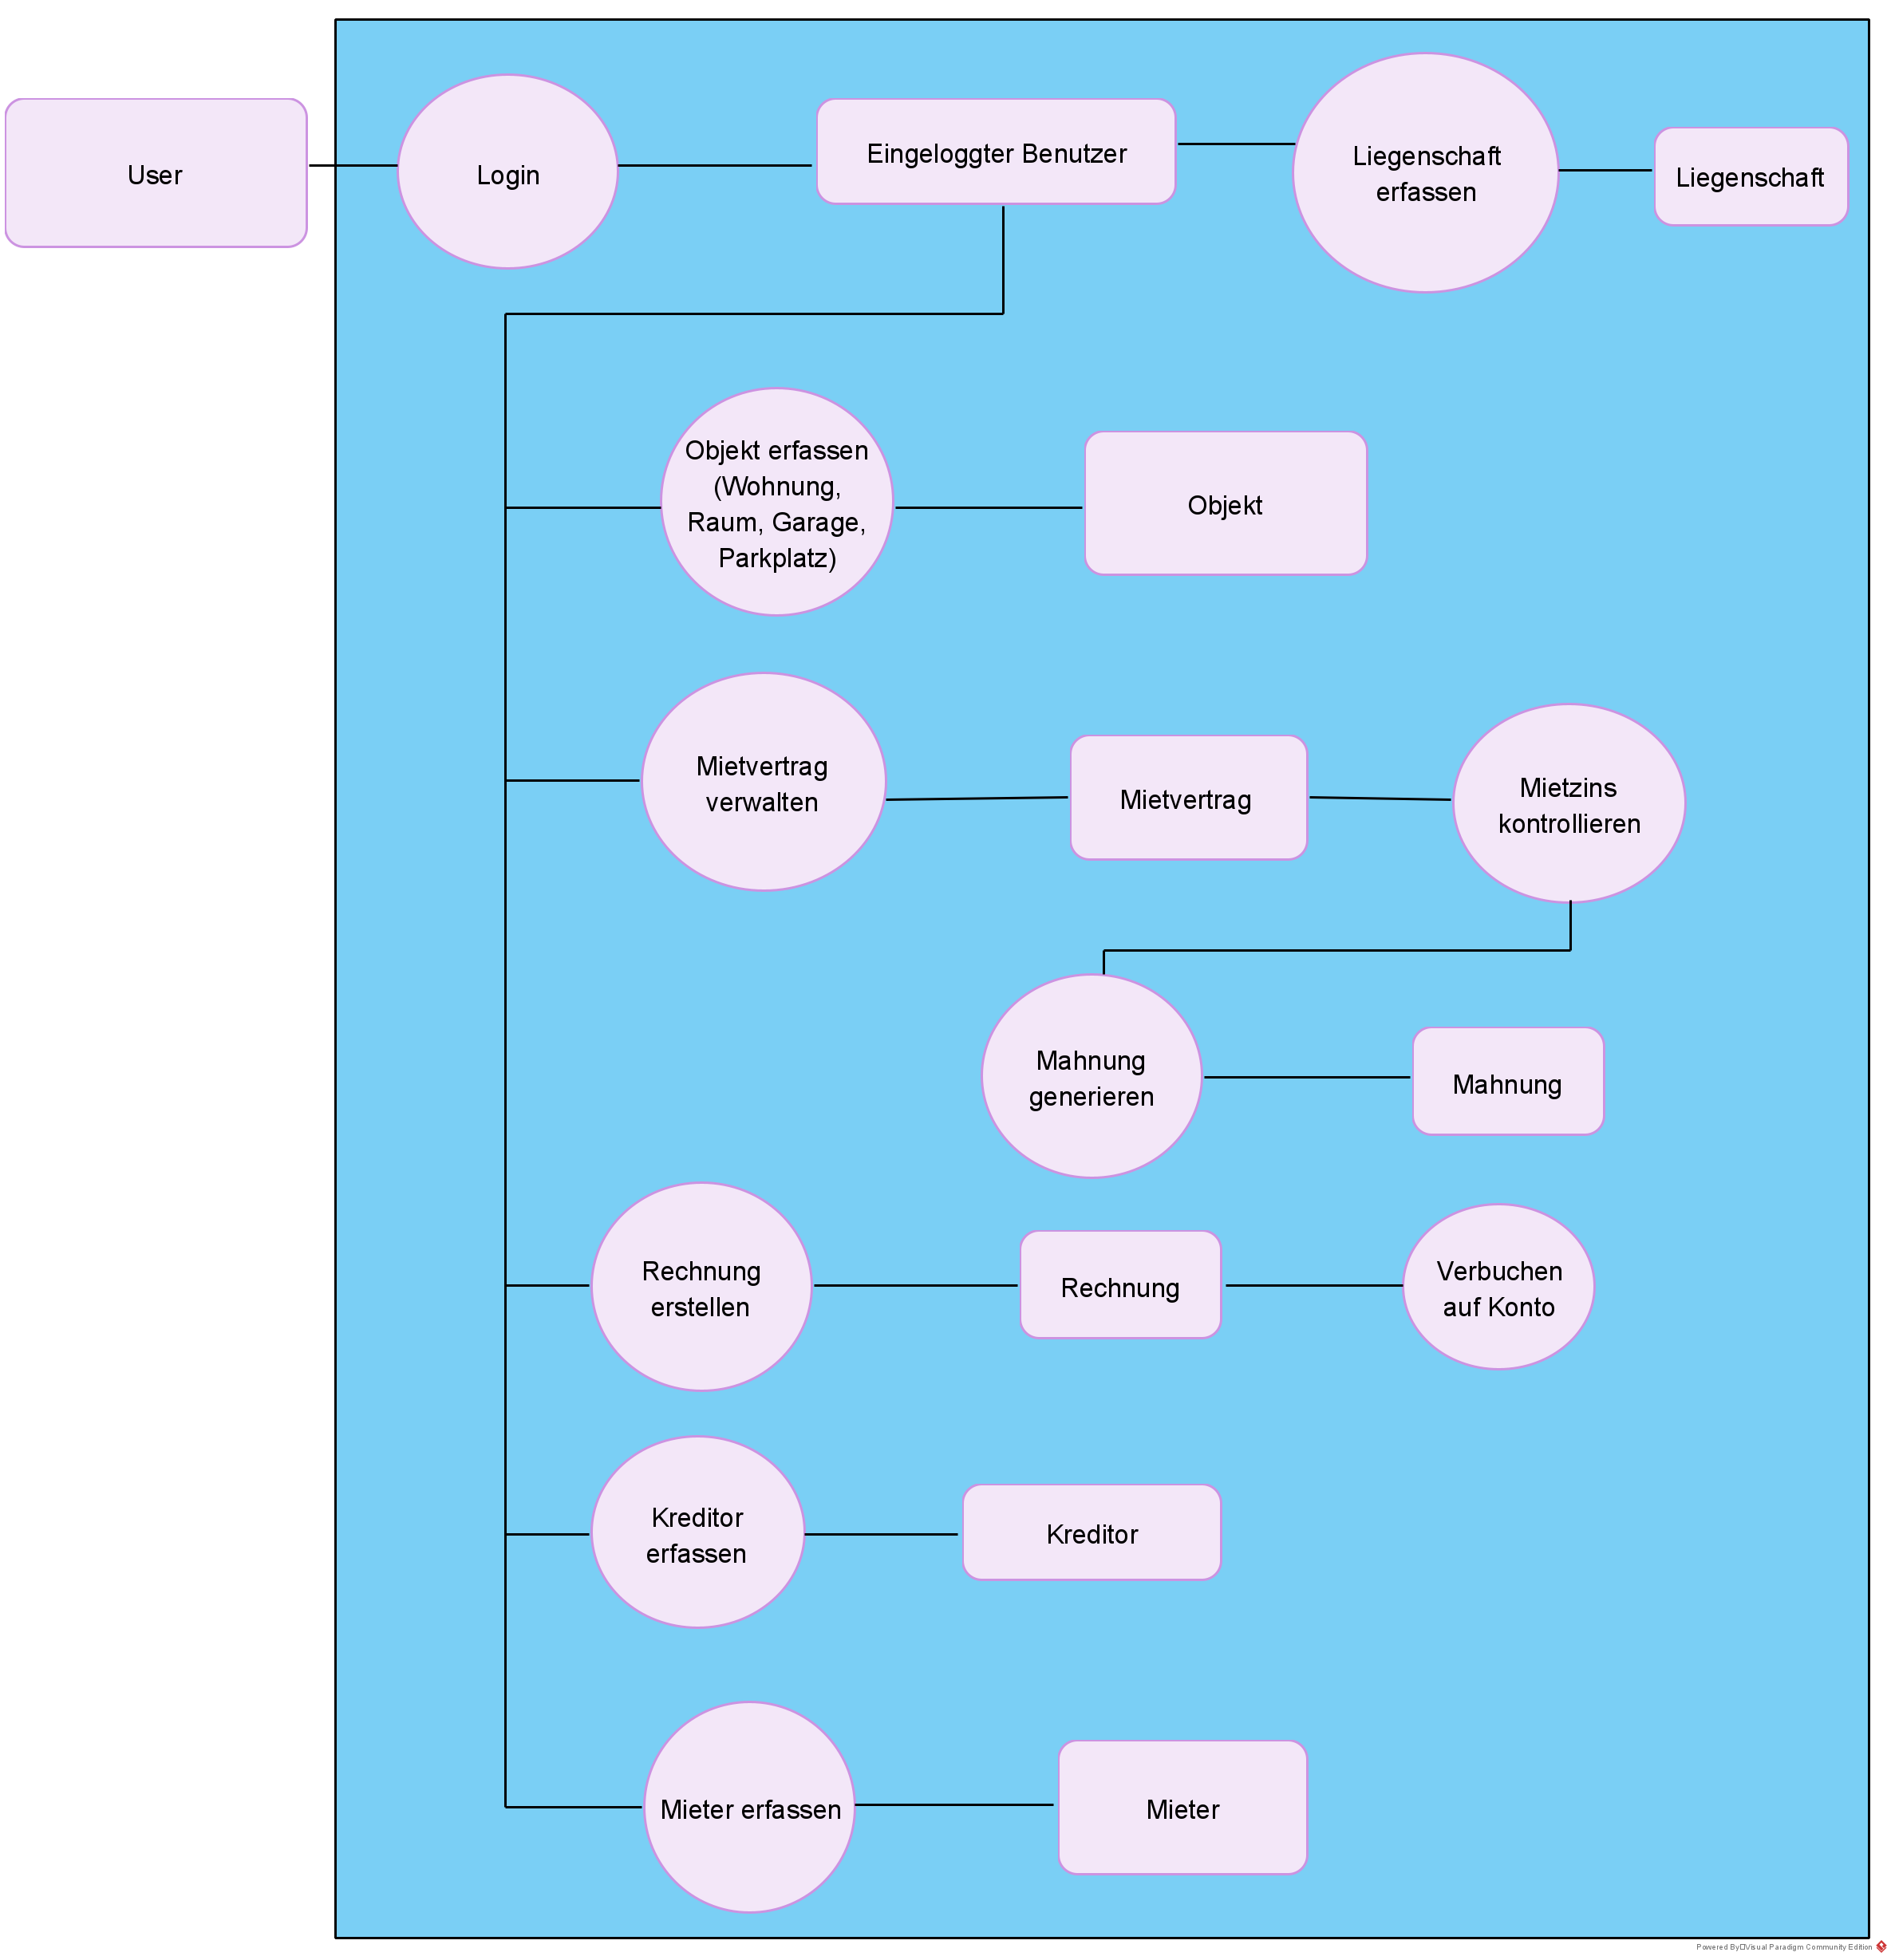
\includegraphics[width=0.99\linewidth]{content/diagrams/out/contextdiagram/context.png}
    \caption{Kontextdiagramm}
  \end{center}
  \label{contextdiag}
\end{figure}

\subsection{Geschäftsprozesse}
\begin{table}[H]
  \newcolumntype{a}{>{\columncolor[HTML]{4473C5}}L}
  \centering
  \settowidth\tymin{\textbf{Kurzbeschreibung}}
  \setlength\extrarowheight{2pt}
  \begin{tabulary}{1.0\textwidth}{|a|m{12cm}|}
    \hline
    \textbf{Name}& Verwaltung von Mietobjekten \\
    \hline 
    \textbf{Kurzbeschreibung} & Alle Geschäftsanwendungsfälle die nötig sid um Mietobjekte korrekt verwalten zu können und im Aufgabenbereich von ImmoGlobal liegen\\
    \hline
    \textbf{Geschäftsanwendungsfälle} & 
    \begin{itemize}
      \item Verwaltung von Objekten
      \item Verwaltung von Liegenschaften
      \item Übernahme- und Übergabeprotokoll der Mietobjekte
      \item Verwaltung der Mieter:innen
      \item Erstellen / Verwalten der Mietverträge
      \item Erfassen von Ein- und Ausgaben  (Mietzins, Nebenkosten, Gebühren für Unterhalt der Liegenschaft, etc.)
      \item Mietzins- und Nebenkostenkontrolle
      \item Rechnung erstellen
    \end{itemize}\\
    \hline
    \textbf{Verantwortlichkeit} & Geschäftsleiter\\
    \hline
    \textbf{Beteiligte} & 
    \begin{itemize}
      \item Mitarbeiter der Administration
      \item Hauswartungspersonen
      \item Mieter
    \end{itemize}\\
    \hline
  \end{tabulary}
  \caption{Geschäftsprozesse}
\end{table}


\subsection{Geschäftsanwendungsfälle}
\begin{table}[H]
  \newcolumntype{a}{>{\columncolor[HTML]{4473C5}}L}
  \centering
  \settowidth\tymin{\textbf{Kurzbeschreibung}}
  \setlength\extrarowheight{2pt}
  \begin{tabulary}{1.0\textwidth}{|a|m{12cm}|}
    \hline
    \textbf{Name}& Verwaltung von Objekten\\
    \hline 
    \textbf{Kurzbeschreibung} & Eine bestehendes Objekt muss editiert werden oder eine neues Objekt soll hinzugefügt werden \\
    \hline
    \textbf{Akteure} & Mitarbeiter in der Liegenschaftsverwaltung\\
    \hline
    \textbf{Auslöser} & Für die erfasste Liegenschaft wurden noch keine Objekte hinzugefügt\newline 
    Ein bestehendes Objekt muss ergänzt/korrigiert werden\\
    \hline
    \textbf{Ergebnis} & Das veränderte oder neu erstellte Objekt kann zu einer Liegenschaft hinzugefügt werden\\
    \hline
    \textbf{Eingehende Daten} & Informationen zum erfassenden Objekt\\
    \hline
    \textbf{Vorbedingungen} & Keine\\
    \hline
    \textbf{Nachbedingungen} & Keine\\
    \hline
    \textbf{Ablauf} & Der Benutzer trägt alle Muss-Daten für das neue Objekt ein und speichert es ab. \\
    \hline
  \end{tabulary}
  \caption{GA-Verwaltung von Objekten}
\end{table}

\begin{table}[H]
  \newcolumntype{a}{>{\columncolor[HTML]{4473C5}}L}
  \centering
  \settowidth\tymin{\textbf{Kurzbeschreibung}}
  \setlength\extrarowheight{2pt}
  \begin{tabulary}{1.0\textwidth}{|a|m{12cm}|}
    \hline
    \textbf{Name}& Verwaltung von Liegenschaften\\
    \hline 
    \textbf{Kurzbeschreibung} & Eine bestehende Liegenschaft muss editiert werden oder eine neue Liegenschaft soll hinzugefügt werden\\
    \hline
    \textbf{Akteure} & Mitarbeiter in der Liegenschaftsverwaltung\\
    \hline
    \textbf{Auslöser} & Die Verwaltung wird mit dem verwalten einer neuen Liegenschaft beauftragt \newline
    Bei einer Liegenschaft müssen Änderungen vorgenommen werden\\
    \hline
    \textbf{Ergebnis} & Die neuen Daten zu der Liegenschaft werden abgespeichert und in der Übersicht dargestellt\\
    \hline
    \textbf{Eingehende Daten} & Liegenschaft mit allen dazu gehörigen Informationen\\
    \hline
    \textbf{Vorbedingungen} & Die Daten zur Liegenschaft müssen bekannt sein\\
    \hline
    \textbf{Nachbedingungen} & Keine\\
    \hline
    \textbf{Ablauf} & Der Eingeloggte Mitarbeiter trägt alle Muss-Daten für die neue Liegenschaft ein und speichert diese. \newline
    Beim editieren einer Liegenschaft wird eine Vorhandene Liegenschaft bearbeitet.\\
    \hline
  \end{tabulary}
  \caption{GA-Verwaltung von Liegenschaften}
\end{table}

\begin{table}[H]
  \newcolumntype{a}{>{\columncolor[HTML]{4473C5}}L}
  \centering
  \settowidth\tymin{\textbf{Kurzbeschreibung}}
  \setlength\extrarowheight{2pt}
  \begin{tabulary}{1.0\textwidth}{|a|m{12cm}|}
    \hline
    \textbf{Name}& Übernahme- und Übergabeprotokoll der Mietobjekte\\
    \hline 
    \textbf{Kurzbeschreibung} & Bei Mietantritt wird ein Übernahmeprotokoll und bei Mietende wird ein Übergabeprotokoll erstellt\\
    \hline
    \textbf{Akteure} & Mitarbeiter in der Liegenschaftsverwaltung, Hauswartungsperson, Mieter\\
    \hline
    \textbf{Auslöser} & Beginn- oder Ende eines Mietverhältnisses\\
    \hline
    \textbf{Ergebnis} & Ein Übernahme- und Übergabeprotokoll für das Mietobjekt\\
    \hline
    \textbf{Eingehende Daten} &  
      $\bullet$ Kündigung \newline
      $\bullet$ Mietvertrag \newline
      $\bullet$ Bei Übergabe zurück an die Verwaltung das Übernahmeprotokoll\\
    \hline
    \textbf{Vorbedingungen} & Keine\\
    \hline
    \textbf{Nachbedingungen} & Keine\\
    \hline
    \textbf{Ablauf} & Für die Übernahme und die Übergabe wird von dem zuständigen Mitarbeiter das Protokoll ausgefüllt und von den Mietparteien auf Vollständigkeit geprüft und unterschrieben. Der Prozess findet komplett Digital statt. Unterschrieben wird das Protokoll auf einem unterschriftsfähigen Tablet. Anschliessend wird daraus ein PDF (PDF/A) generiert und dem Mieter wahlweise per E-Mail oder ausgedruckt per Post zugesandt\\
    \hline
  \end{tabulary}
  \caption{GA-Übernahme- und Übergabeprotokoll der Mietobjekte}
\end{table}

\begin{table}[H]
  \newcolumntype{a}{>{\columncolor[HTML]{4473C5}}L}
  \centering
  \settowidth\tymin{\textbf{Kurzbeschreibung}}
  \setlength\extrarowheight{2pt}
  \begin{tabulary}{1.0\textwidth}{|a|m{12cm}|}
    \hline
    \textbf{Name}& Verwaltung der Mieter:innen\\
    \hline 
    \textbf{Kurzbeschreibung} & Neue Mieter:innen werden in der Applikation hinzugefügt oder bestehende Mieter:innen bearbeitet\\
    \hline
    \textbf{Akteure} & Mitarbeiter in der Liegenschaftsverwaltung, Mieter\\
    \hline
    \textbf{Auslöser} & 
      $\bullet$ Vermietung eines Objektes an einen neuen Mieter:in \newline
      $\bullet$ Namensänderungen \newline
      $\bullet$ Zivilstandänderungen \newline
      $\bullet$ Geburten\\
    \hline
    \textbf{Ergebnis} &
      $\bullet$ Ein neuer Mieter:in wurde in der Applikation erfasst \newline
      $\bullet$ Änderung an bestehendem Mieter:in wurden durchgeführt\\
    \hline
    \textbf{Eingehende Daten} & Informationen über den Mieter:in\\
    \hline
    \textbf{Vorbedingungen} & Die Informationen über den Mieter:in müssen bekannt sein\\
    \hline
    \textbf{Nachbedingungen} & Keine\\
    \hline
    \textbf{Ablauf} & Der Benutzer der Applikation erstellt einen neuen Mieter:in. Er gibt alle Informationen ein und Speichert die Daten ab. Bei einer Änderung eines bestehenden Mieter:in, wird dieser in der Applikation gesucht und ausgewählt, editiert und abgespeichert\\
    \hline
  \end{tabulary}
  \caption{GA-Verwaltung der Mieter:innen}
\end{table}

\begin{table}[H]
  \newcolumntype{a}{>{\columncolor[HTML]{4473C5}}L}
  \centering
  \settowidth\tymin{\textbf{Kurzbeschreibung}}
  \setlength\extrarowheight{2pt}
  \begin{tabulary}{1.0\textwidth}{|a|m{12cm}|}
    \hline
    \textbf{Name}& Erstellen / Verwalten der Mietverträge\\
    \hline 
    \textbf{Kurzbeschreibung} & \\
    \hline
    \textbf{Akteure} & Mitarbeiter in der Liegenschaftsverwaltung, Mieter:in\\
    \hline
    \textbf{Auslöser} & Bewerbung eines neuen Mieters wurde akzeptiert\\
    \hline
    \textbf{Ergebnis} & Gültiger (unterschriebener) Mietvertrag\\
    \hline
    \textbf{Eingehende Daten} & 
      $\bullet$ Bewerbung mit allen Daten zum zukünftigen Mieter \newline
      $\bullet$ Betreibungsregisterauszug\\
    \hline
    \textbf{Vorbedingungen} & 
      $\bullet$ Bewerbung des Mieters wurde akzeptiert \newline
      $\bullet$ Bonität des Mieters wurde überprüft\\
    \hline
    \textbf{Nachbedingungen} & Keine\\
    \hline
    \textbf{Ablauf} & Der Benutzer der Applikation erstellt im betreffenden Mietobjekt einen neuen Mietvertrag. Den Mieter wählt er aus der Liste der vorhandenen Mieter aus. Falls der neue Mieter noch nicht erfasst wurde, kann er diesen erstellen. Anschliessend wird der neue Mietvertrag ausgedruckt und kann von beiden Parteien unterschrieben werden. Nachdem der Mietvertrag unterschrieben ist, wird dieser als PDF in der Applikation abgelegt und als Gültig markiert. Bei einer Kündigung des Mietverhältnisses wird die Kündigung des Mietvertrags in die Applikation hochgeladen und der der Status auf gekündigt geändert. Sobald dann das ende des Mietverhältnisses erreicht ist, wird der Status auf beendet gesetzt.\\
    \hline
  \end{tabulary}
  \caption{GA-Erstellen / Verwalten der Mietverträge}
\end{table}

\begin{table}[H]
  \newcolumntype{a}{>{\columncolor[HTML]{4473C5}}L}
  \centering
  \settowidth\tymin{\textbf{Kurzbeschreibung}}
  \setlength\extrarowheight{2pt}
  \begin{tabulary}{1.0\textwidth}{|a|m{12cm}|}
    \hline
    \textbf{Name}& Erfassen von Ein- und Ausgaben\\
    \hline 
    \textbf{Kurzbeschreibung} & Alle Einnahmen und alle Ausgaben werden erfasst\\
    \hline
    \textbf{Akteure} & Mitarbeiter in der Liegenschaftsverwaltung\\
    \hline
    \textbf{Auslöser} & Zahlungs-Eingang / Ausgang\\
    \hline
    \textbf{Ergebnis} & Neuer Zahlungs-Ein/Ausgang ist im System erfasst\\
    \hline
    \textbf{Eingehende Daten} &
      $\bullet$ Rechnungen \newline
      $\bullet$ Abrechnungen\\
    \hline
    \textbf{Vorbedingungen} & Keine\\
    \hline
    \textbf{Nachbedingungen} & Keine\\
    \hline
    \textbf{Ablauf} & Der Benutzer trägt alle Zahlungseingänge im System ein. Wenn eine Zahlung anhand einer Rechnung getätigt werden muss, bezahlt er diese und trägt den Rechnungsbetrag ebenfalls im System ein\\
    \hline
  \end{tabulary}
  \caption{GA-Kreditor erfassen}
\end{table}

\begin{table}[H]
  \newcolumntype{a}{>{\columncolor[HTML]{4473C5}}L}
  \centering
  \settowidth\tymin{\textbf{Kurzbeschreibung}}
  \setlength\extrarowheight{2pt}
  \begin{tabulary}{1.0\textwidth}{|a|m{12cm}|}
    \hline
    \textbf{Name}&Mietzins- und Nebenkostenkontrolle\\
    \hline 
    \textbf{Kurzbeschreibung} & Der Eingang der Mietzinse und der Nebenkostenzahlungen wird kontrolliert und bei fehlenden Eingängen wird eine Mahnung erstellt\\
    \hline
    \textbf{Akteure} & Mitarbeiter in der Liegenschaftsverwaltung\\
    \hline
    \textbf{Auslöser} & Mietzins- und Nebenkostenzahlungsüberprüfung\\
    \hline
    \textbf{Ergebnis} & Bei negativer Prüfung eine Mahnung\newline 
    Bei positiver Prüfung nichts\\
    \hline
    \textbf{Eingehende Daten} & Mietvertrag\\
    \hline
    \textbf{Vorbedingungen} & Es müssen gültige Mietverträge im System erfasst sein \\
    \hline
    \textbf{Nachbedingungen} & Keine \\
    \hline
    \textbf{Ablauf} & Der Benutzer überprüft, ob für ein entsprechendes Objekt die Miete und die Nebenkosten bezahlt wurden. Wenn die Miete oder die Nebenkosten noch nicht bezahlt wurden, kann er eine Mahnung generieren und ausdrucken.\\
    \hline
  \end{tabulary}
  \caption{GA-Mietzins- und Nebenkostenkontrolle}
\end{table}

\begin{table}[H]
  \newcolumntype{a}{>{\columncolor[HTML]{4473C5}}L}
  \centering
  \settowidth\tymin{\textbf{Kurzbeschreibung}}
  \setlength\extrarowheight{2pt}
  \begin{tabulary}{1.0\textwidth}{|a|m{12cm}|}
    \hline
    \textbf{Name}&Rechnung erstellen\\
    \hline 
    \textbf{Kurzbeschreibung} & Eine neue Rechnung erstellen\\
    \hline
    \textbf{Akteure} & Mitarbeiter in der Liegenschaftsverwaltung\\
    \hline
    \textbf{Auslöser} & Es wurde eine Dienstleistung, die die Liegenschaftsverwaltung getätigt hat, bezogen \newline 
    Für eine Liegenschaft oder ein Objekt wurde die Nebenkostenabrechnung erstellt\\
    \hline
    \textbf{Ergebnis} & Eine Rechnung die nach dem freigeben nicht mehr bearbeitet werden kann\\
    \hline
    \textbf{Eingehende Daten} & Informationen warum die Rechnung erstellt werden muss \\
    \hline
    \textbf{Vorbedingungen} & Keine\\
    \hline
    \textbf{Nachbedingungen} & Keine\\
    \hline
    \textbf{Ablauf} & Der Benutzer erstellt eine neue Rechnung und gibt alle nötigen Informationen für die Rechnung ein. Der Benutzer ordnet die Rechnung einem bestimmten Konto zu. Falls das Konto noch nicht besteht, muss dieses zuerst noch erstellt werden. Wenn die Rechnung für den Kreditor/Mieter freigegeben wird, ändert der Status der Rechnung auf ''freigeben'' und kann nicht mehr abgeändert werden. Wenn nach der Freigabe Fehler bemerkt werden, muss der Status der Rechnung auf Storniert gewechselt werden und eine neue Rechnung erstellt werden. Der Benutzer hat aber auch die Möglichkeit, die Rechnung nicht freizugeben und die Bearbeitung zu einem späteren Zeitpunkt fortzusetzen.\\
    \hline
  \end{tabulary}
  \caption{GA-Rechnung erstellen}
  \label{GA-rechnungErstellen}
\end{table}

\subsection{Use-Case-Beschreibungen}

\begin{figure}[H]
  \begin{center}
    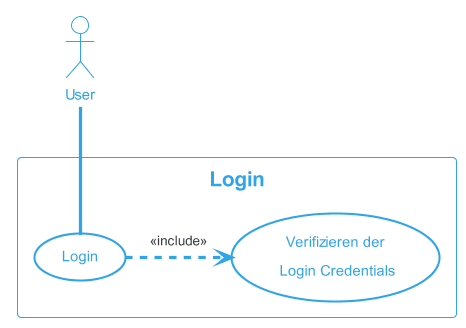
\includegraphics[width=0.6\linewidth]{content/diagrams/out/usecase/login/Login.png}
    \caption{UC-Login}
    \label{login}
  \end{center}
\end{figure}

\begin{table}[H]
  \newcolumntype{a}{>{\columncolor[HTML]{4473C5}}L}
  \centering
  \settowidth\tymin{\textbf{Kurzbeschreibung}}
  \setlength\extrarowheight{2pt}
  \begin{tabulary}{1.0\textwidth}{|a|m{14cm}|}
    \hline
    \textbf{Name}& Login\\
    \hline
    \textbf{Akteur}& Mitarbeiter:in der Liegenschaftsverwaltung, Hauswartungspersonen, Geschäftsführer\\
    \hline 
    \textbf{Beschreibung} & Ein Akteur will sich in der Applikation anmelden\\
    \hline
    \textbf{Daten} & Login-Daten des Benutzers\\
    \hline
    \textbf{Auslöser} & Benutzerbefehl der von dem entsprechenden Akteur initiiert wird\\
    \hline
    \textbf{Antwort} & Bestätigung, dass das Login erfolgreich war\\
    \hline
    \textbf{Kommentare} & -\\
    \hline
  \end{tabulary}
  \caption{UC-Login}
\end{table}

\begin{figure}[H]
  \begin{center}
    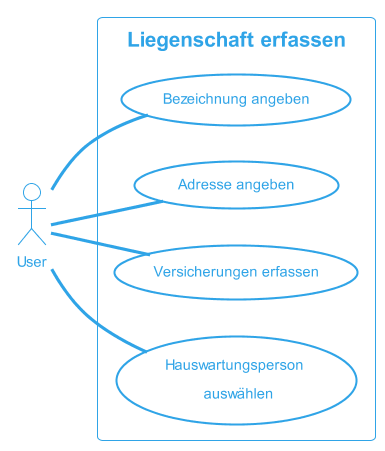
\includegraphics[width=0.43\linewidth]{content/diagrams/out/usecase/liegenschaftErfassen/LiegenschaftErfassen.png}
    \caption{UC-Liegenschaft erfassen}
    \label{Liegenschaft}
  \end{center}
\end{figure}

\vspace*{-1cm}

\begin{table}[H]
  \newcolumntype{a}{>{\columncolor[HTML]{4473C5}}L}
  \centering
  \settowidth\tymin{\textbf{Kurzbeschreibung}}
  \setlength\extrarowheight{2pt}
  \begin{tabulary}{1.0\textwidth}{|a|m{14cm}|}
    \hline
    \textbf{Name}& Liegenschaft erfassen\\
    \hline
    \textbf{Akteur}& Mitarbeiter:in der Liegenschaftsverwaltung\\
    \hline 
    \textbf{Beschreibung} & Der zuständige Mitarbeiter:in loggt sich in der Applikation ein und kann anschliessend die Liegenschaft über einen Button erfassen. Es müssen alle Daten zur Liegenschaft eingetragen werden sonst kann der Mitarbeiter die Liegenschaft nicht abspeichern.\\
    \hline
    \textbf{Daten} & Informationen zur Liegenschaft\\
    \hline
    \textbf{Auslöser} & Benutzerbefehl der von dem entsprechenden Akteur initiiert wird\\
    \hline
    \textbf{Antwort} & Bestätigung, dass das erfassen der Liegenschaft erfolgreich war\\
    \hline
    \textbf{Kommentare} & Bei fehlenden Angaben wird dem Benutzer eine Fehlermeldung angezeigt\\
    \hline
  \end{tabulary}
  \caption{UC-Liegenschaft erfassen}
\end{table}

\begin{figure}[H]
  \begin{center}
    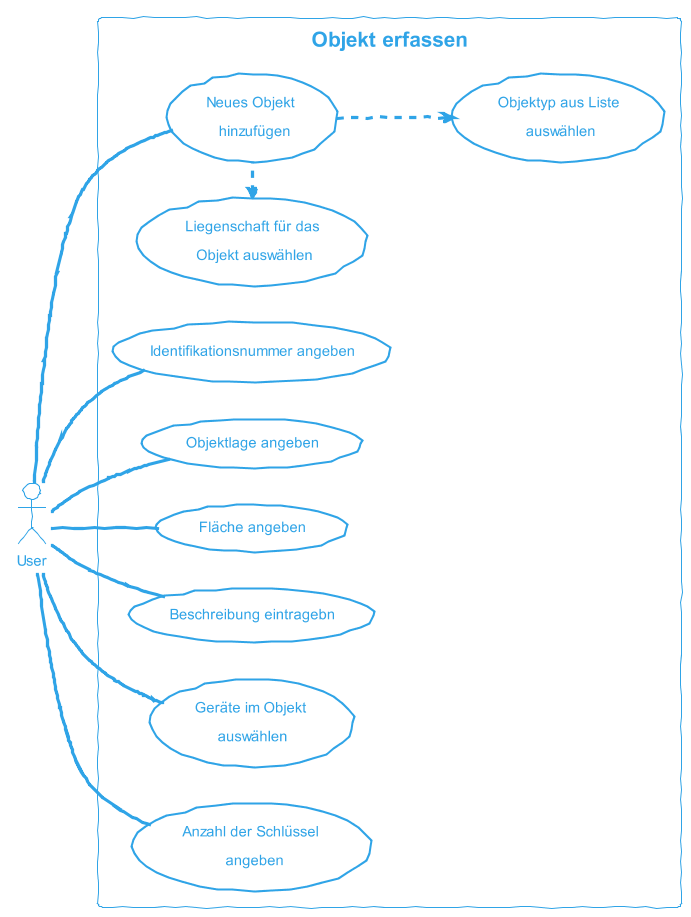
\includegraphics[width=0.8\linewidth]{content/diagrams/out/usecase/objektErfassen/ObjektErfassen.png}
    \caption{UC-Objekt erfassen}
    \label{objekt}
  \end{center}
\end{figure}

\vspace*{-1cm}

\begin{table}[H]
  \newcolumntype{a}{>{\columncolor[HTML]{4473C5}}L}
  \centering
  \settowidth\tymin{\textbf{Kurzbeschreibung}}
  \setlength\extrarowheight{2pt}
  \begin{tabulary}{1.0\textwidth}{|a|m{14cm}|}
    \hline
    \textbf{Name}& Objekt erfassen\\
    \hline
    \textbf{Akteur}& Mitarbeiter:in der Liegenschaftsverwaltung\\
    \hline 
    \textbf{Beschreibung} & Der zuständige Mitarbeiter:in loggt sich in der Applikation ein und kann anschliessend das Objekt über einen Button erfassen. Es müssen alle Daten zum Objekt eingetragen werden sonst kann dieses nicht abgespeichert werden\\
    \hline
    \textbf{Daten} & Informationen zum Objekt\\
    \hline
    \textbf{Auslöser} & Benutzerbefehl der von dem entsprechenden Akteur initiiert wird\\
    \hline
    \textbf{Antwort} & Bestätigung, dass das erfassen des Objektes erfolgreich war\\
    \hline
    \textbf{Kommentare} & Bei fehlenden Angaben wird dem Benutzer eine Fehlermeldung angezeigt\newline 
    Ein Objekt kann nur über eine Liegenschaft erfasst werden\\
    \hline
  \end{tabulary}
  \caption{UC-Objekt erfassen}
\end{table}

\begin{figure}[H]
  \begin{center}
    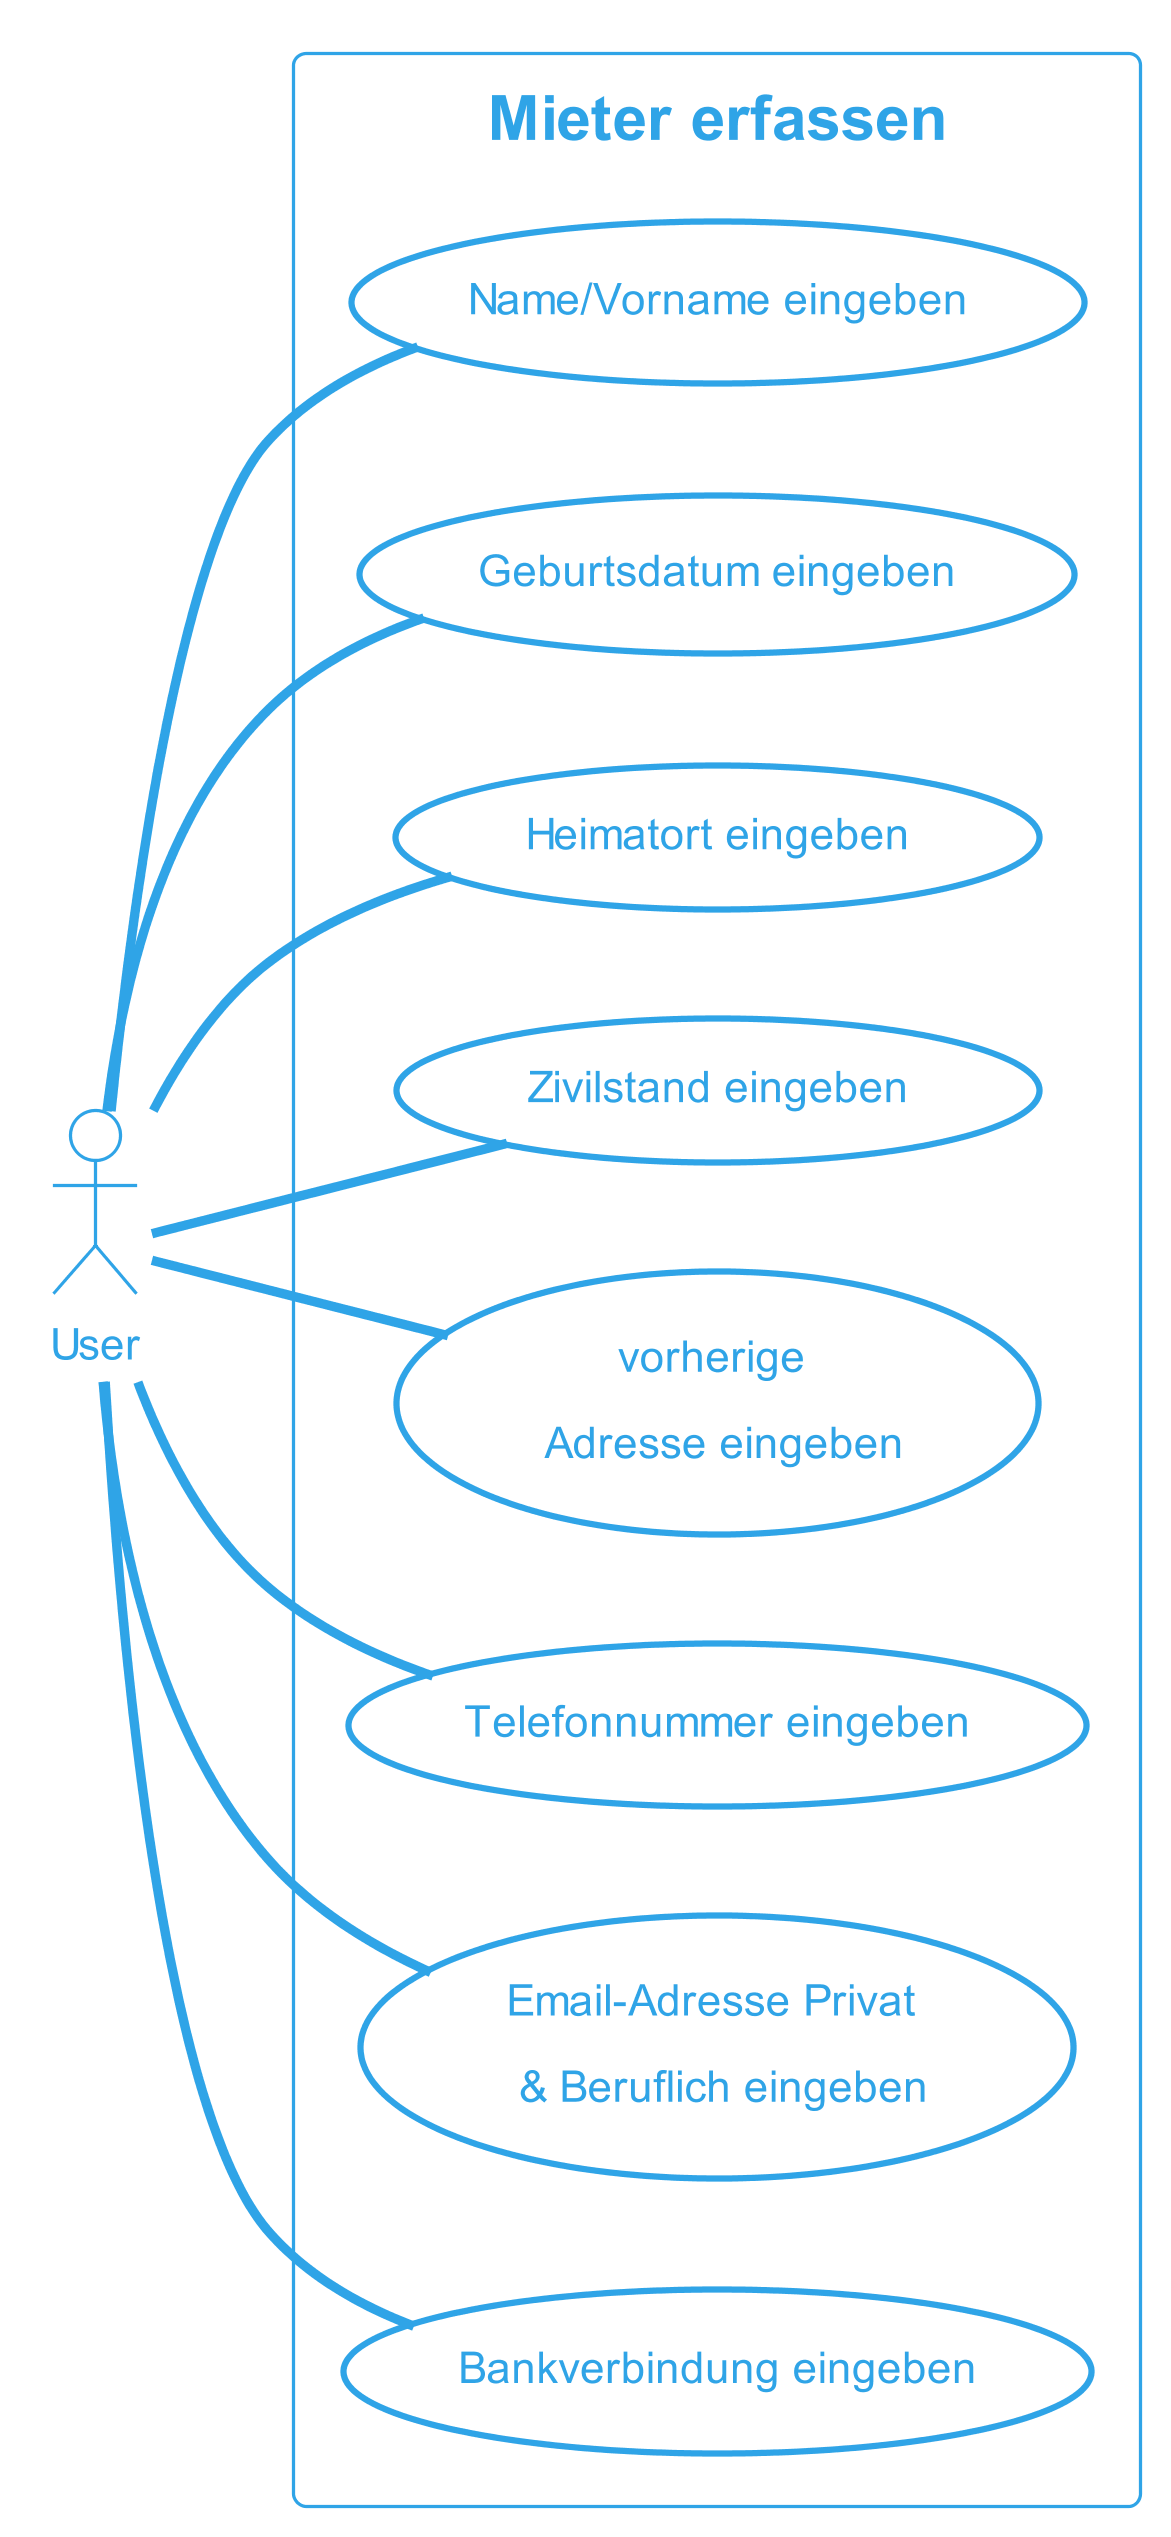
\includegraphics[width=0.4\linewidth]{content/diagrams/out/usecase/mieterErfassen/Mieter erfassen.png}
    \caption{UC-Mieter:in erfassen}
    \label{mieterErfassen}
  \end{center}
\end{figure}

\begin{table}[H]
  \newcolumntype{a}{>{\columncolor[HTML]{4473C5}}L}
  \centering
  \settowidth\tymin{\textbf{Kurzbeschreibung}}
  \setlength\extrarowheight{2pt}
  \begin{tabulary}{1.0\textwidth}{|a|m{14cm}|}
    \hline
    \textbf{Name}& Mieter:in erfassen\\
    \hline
    \textbf{Akteur}& Mitarbeiter:in der Liegenschaftsverwaltung\\
    \hline 
    \textbf{Beschreibung} & Wird die Bewerbung eines Mieters für ein Objekt angenommen, muss dieser Mieter:in in der Applikation erfasst werden. Der zuständige Mitarbeiter:in loggt sich dazu in der Applikation ein und kann den Mieter:in im entsprechenden Formular erfassen\\
    \hline
    \textbf{Daten} & Vollständige Daten zum Mieter\\
    \hline
    \textbf{Auslöser} & Benutzerbefehl der von dem entsprechenden Akteur initiiert wird\\
    \hline
    \textbf{Antwort} & Bestätigung, dass der Mieter erfolgreich erfasst wurde\\
    \hline
    \textbf{Kommentare} & -\\
    \hline
  \end{tabulary}
  \caption{UC-Mieter:in erfassen}
\end{table}

\begin{figure}[H]
  \begin{center}
    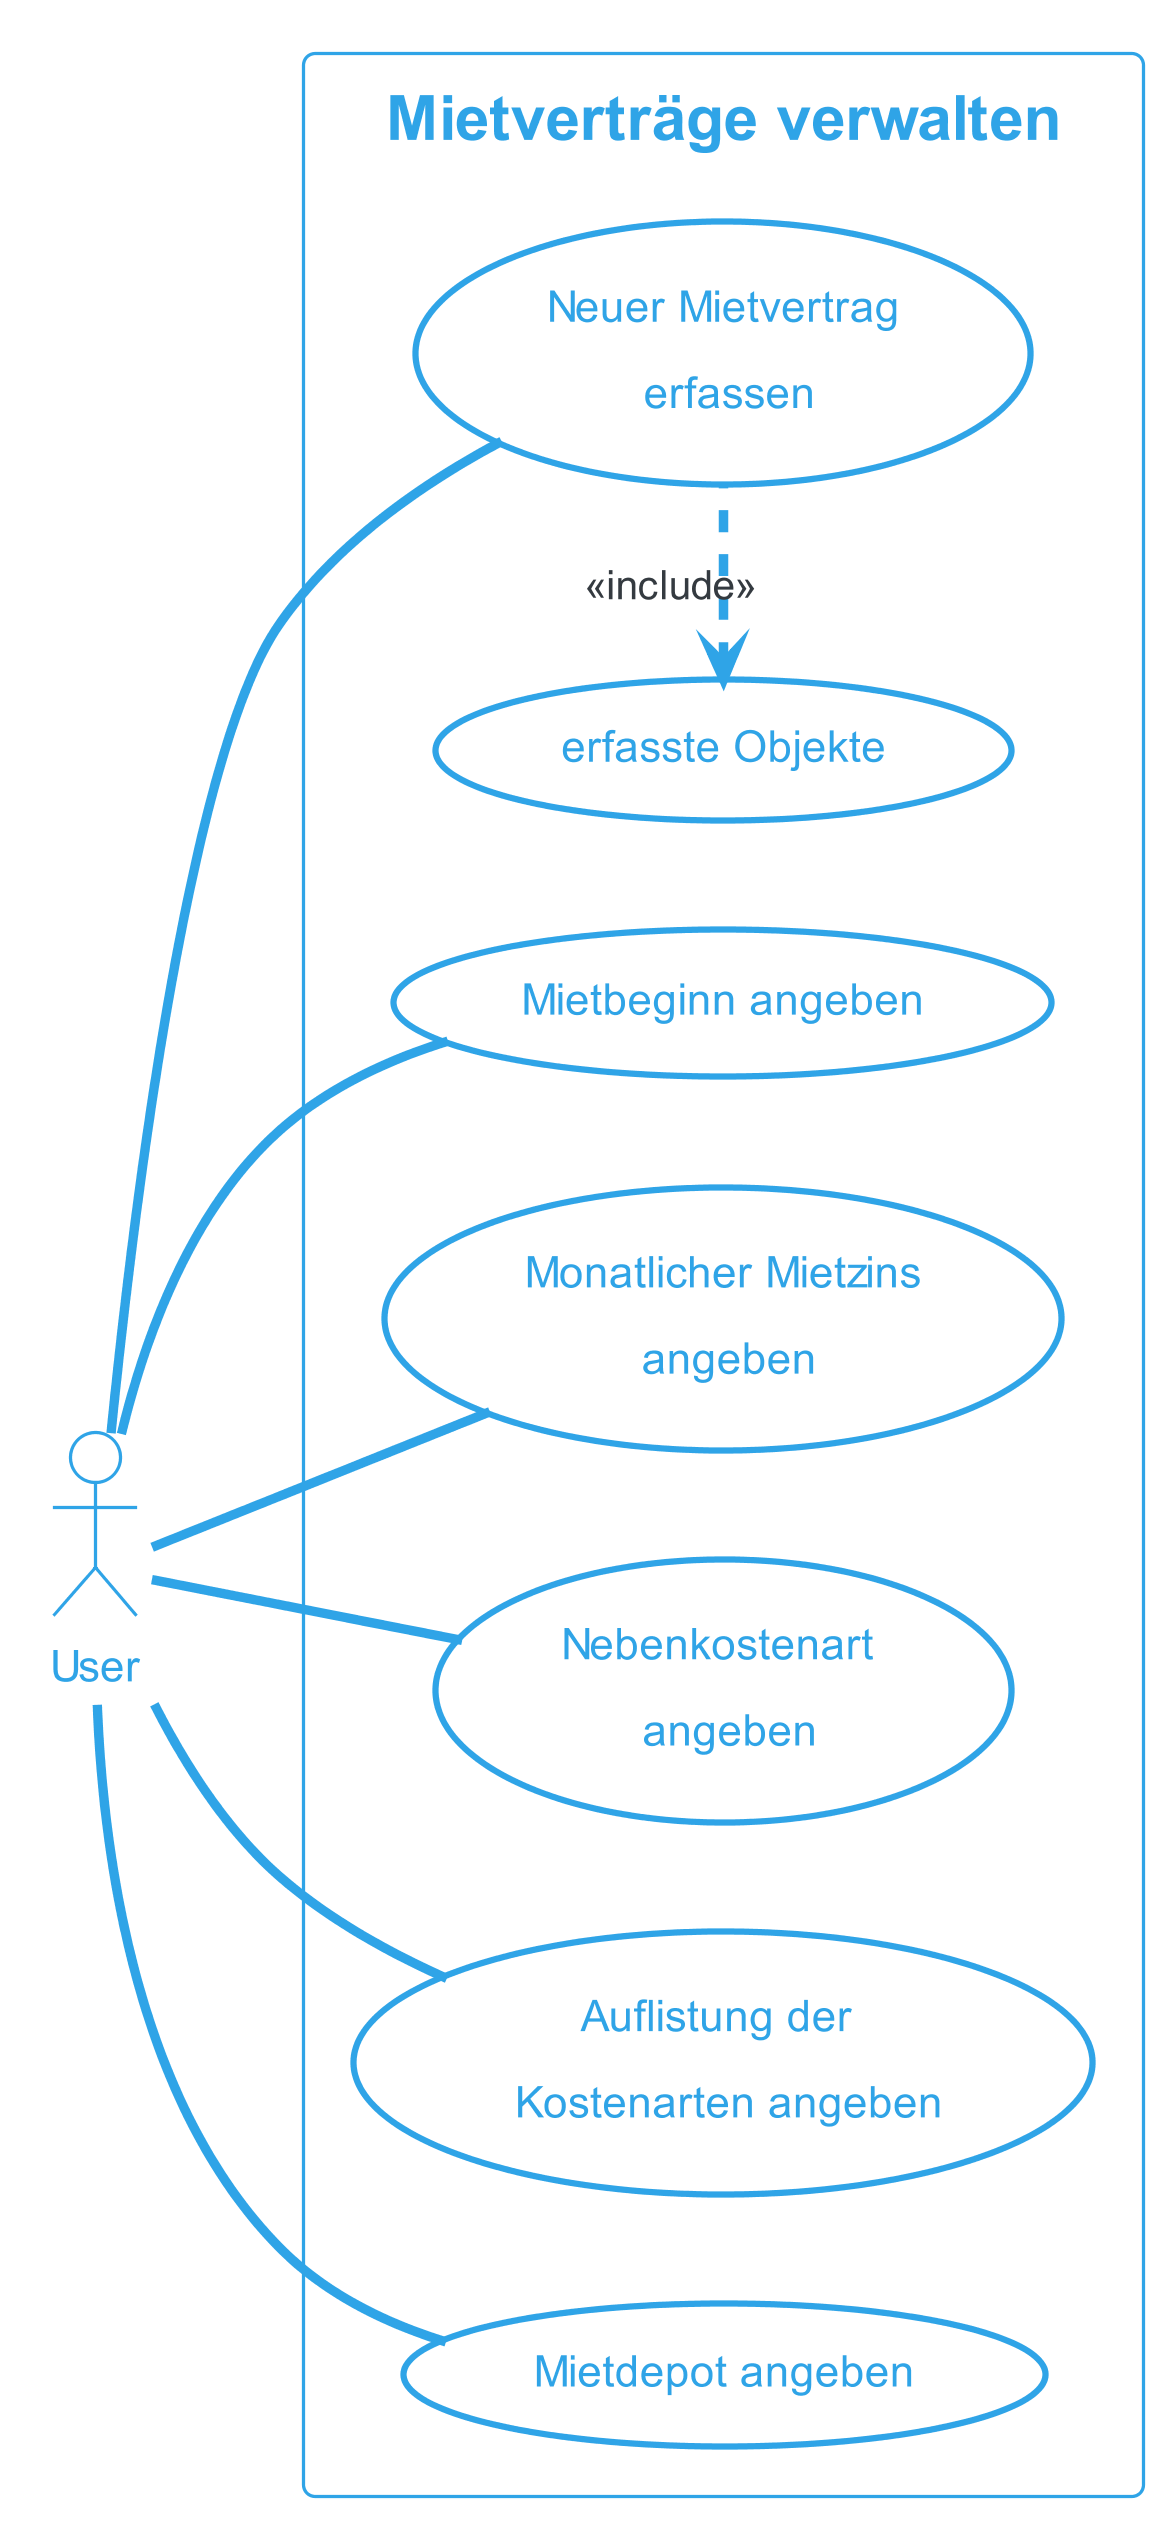
\includegraphics[width=0.43\linewidth]{content/diagrams/out/usecase/mietverträgeVerwalten/MietverträgeVerwalten.png}
    \caption{UC-Mietverträge verwalten}
    \label{MietvertraegeVerwalten}
  \end{center}
\end{figure}

\vspace*{-1cm}

  \begin{table}[H]
    \newcolumntype{a}{>{\columncolor[HTML]{4473C5}}L}
    \centering
    \settowidth\tymin{\textbf{Kurzbeschreibung}}
    \setlength\extrarowheight{2pt}
      \begin{tabulary}{1.0\textwidth}{|a|m{14cm}|}
        \hline
        \textbf{Name}& Mietverträge verwalten\\
      \hline
      \textbf{Akteur}& Mitarbeiter:in der Liegenschaftsverwaltung\\
      \hline 
      \textbf{Beschreibung} & Der zuständige Mitarbeiter:in loggt sich in der Applikation ein und erstellt anschliessend einen neuen Mietvertrag der noch den Status ungültig hat, bis dieser von beiden Parteien unterschrieben wurde\\
      \hline
      \textbf{Daten} & Alle Daten die zum erfassen des Mietvertrags nötig sind \\
      \hline
      \textbf{Auslöser} & Benutzerbefehl der von dem entsprechenden Akteur initiiert wird\\
      \hline
      \textbf{Antwort} & Bestätigung, dass der Mietvertrag erfolgreich erfasst wurde und ausgedruckt werden kann\\
      \hline
      \textbf{Kommentare} & Bei fehlenden Angaben wird dem Benutzer eine Fehlermeldung angezeigt\\
      \hline
  \end{tabulary}
  \caption{UC-Mietverträge verwalten}
  \end{table}

\begin{figure}[H]
  \begin{center}
    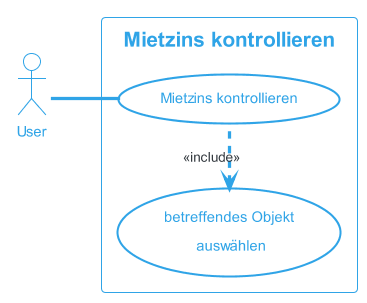
\includegraphics[width=0.4\linewidth]{content/diagrams/out/usecase/mietzinsKontrollieren/MietzinsKontrollieren.png}
    \caption{UC-Mietzins kontrollieren}
    \label{MietzinsKontrollieren}
  \end{center}
\end{figure}

\begin{table}[H]
  \newcolumntype{a}{>{\columncolor[HTML]{4473C5}}L}
  \centering
  \settowidth\tymin{\textbf{Kurzbeschreibung}}
  \setlength\extrarowheight{2pt}
  \begin{tabulary}{1.0\textwidth}{|a|m{14cm}|}
    \hline
    \textbf{Name}& Mietzins kontrollieren\\
    \hline
    \textbf{Akteur}& Mitarbeiter:in der Liegenschaftsverwaltung\\
    \hline 
    \textbf{Beschreibung} & Wenn die Zahlungen geprüft werden müssen, loggt sich der zuständige Mitarbeiter:in ein und kann auf dem entsprechenden Objekt Kontrollieren ob die Miete oder die Nebenkosten schon als ''bezahlt'' markiert wurde\\
    \hline
    \textbf{Daten} & Zu prüfendes Objekt\\
    \hline
    \textbf{Auslöser} & Benutzerbefehl der von dem entsprechenden Akteur initiiert wird\\
    \hline
    \textbf{Antwort} & Zahlungen wurde getätigt oder im Verzug\\
    \hline
    \textbf{Kommentare} & Bei Zahlungen im Verzug wird der nächste UseCase \fref{mahnung} eingesetzt\\
    \hline
  \end{tabulary}
  \caption{UC-Mietzins kontrollieren}
\end{table}

\newpage

\begin{figure}[H]
  \begin{center}
    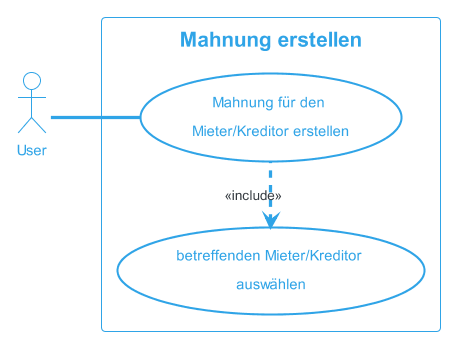
\includegraphics[width=0.5\linewidth]{content/diagrams/out/usecase/mahnungGenerieren/MahnungErstellen.png}
    \caption{UC-Mahnung erstellen}
    \label{mahnung}
  \end{center}
\end{figure}

\begin{table}[H]
  \newcolumntype{a}{>{\columncolor[HTML]{4473C5}}L}
  \centering
  \settowidth\tymin{\textbf{Kurzbeschreibung}}
  \setlength\extrarowheight{2pt}
  \begin{tabulary}{1.0\textwidth}{|a|m{14cm}|}
    \hline
    \textbf{Name}& Mahnung erstellen\\
    \hline
    \textbf{Akteur}& Mitarbeiter:in der Liegenschaftsverwaltung\\
    \hline 
    \textbf{Beschreibung} & Fällt die Prüfung der Mietzins-oder Nebenkostenzahlung negativ aus, kann der Benutzer eine Mahnung für den Mieter erstellen \\
    \hline
    \textbf{Daten} & Rechnungsbetrag\\
    \hline
    \textbf{Auslöser} & Benutzerbefehl der von dem entsprechenden Akteur initiiert wird\\
    \hline
    \textbf{Antwort} & Bestätigung, dass die Mahnung erfolgreich erstellt wurde und jetzt ausgedruckt werden kann\\
    \hline
    \textbf{Kommentare} & Normalerweise ist der zuständige Mitarbeiter:in in der Applikation schon eingeloggt da er die Prüfung der Zahlung vorgenommen hatte. Das erstellen der Mahnung wird dann direkt von dort aus ausgelöst\\
    \hline
  \end{tabulary}
  \caption{UC-Mahnung erstellen}
\end{table}

\begin{figure}[H]
  \begin{center}
    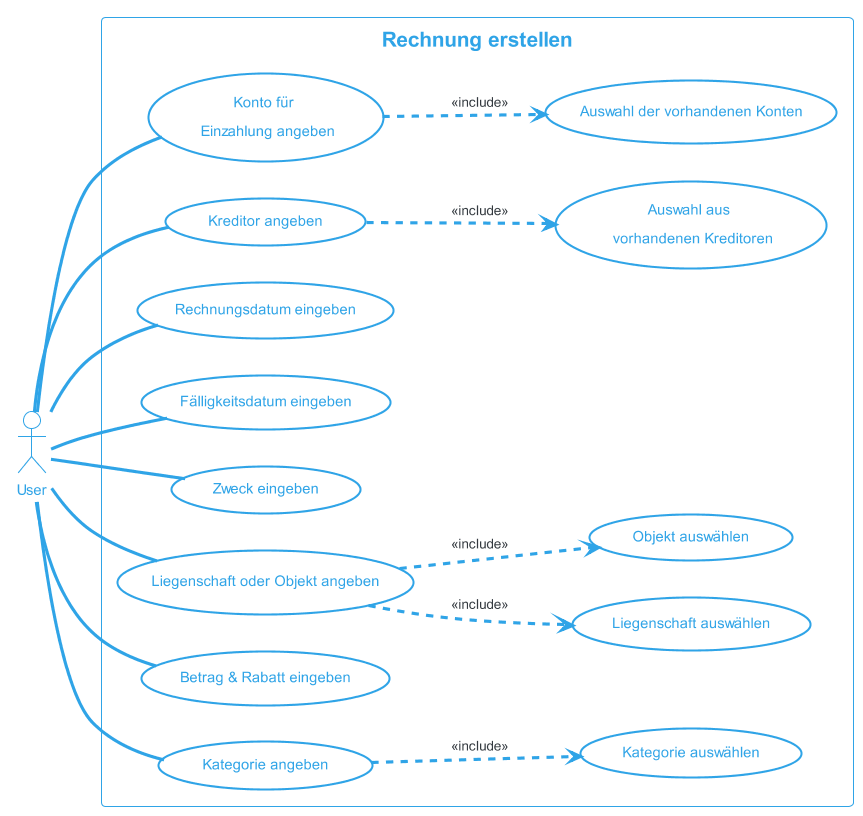
\includegraphics[width=0.85\linewidth]{content/diagrams/out/usecase/rechnungErstellen/Rechnung erstellen.png}
    \caption{UC-Rechnung erstellen}
    \label{RechnungErstellen}
  \end{center}
\end{figure}
\vspace*{-1.2cm}
\begin{table}[H]
  \newcolumntype{a}{>{\columncolor[HTML]{4473C5}}L}
  \centering
  \settowidth\tymin{\textbf{Kurzbeschreibung}}
  \setlength\extrarowheight{2pt}
  \begin{tabulary}{1.0\textwidth}{|a|m{14cm}|}
    \hline
    \textbf{Name}& Rechnung erstellen\\
    \hline
    \textbf{Akteur}& Mitarbeiter:in der Liegenschaftsverwaltung\\
    \hline 
    \textbf{Beschreibung} & Um eine Rechnung zu erstellen, muss sich der Zuständige Mitarbeiter:in in der Applikation einloggen. Es kann dann für eine Dienstleistung eine Rechnung erstellt werden. Um die Rechnung für eine Dienstleistung zu erstellen, müssen alle Daten eingegeben werden \newline 
    Wird eine Rechnung für die fällige Miete oder die Nebenkosten erstellt, werden die Daten für die Rechnung aus der angewählten Liegenschaft oder Objekt in die Rechnung eingefügt. Allfällige Anpassungen können nachträglichen als separate Rechnungsposition hinzugefügt werden \newline
    Die Rechnungen werden immer einem Konto zugeordnet. Falls das gewünschte Konto noch nicht besteht, muss es noch erstellt werden\\
    \hline
    \textbf{Daten} &       
      $\bullet$ Kreditor\newline
      $\bullet$ Rechnungsbetrag \newline
      $\bullet$ Objekt oder Liegenschaft\\
    \hline
    \textbf{Auslöser} & Benutzerbefehl der von dem entsprechenden Akteur initiiert wird\\
    \hline
    \textbf{Antwort} & Bestätigung, dass die Rechnung erfolgreich erstellt wurde und ausgedruckt werden kann\\
    \hline
    \textbf{Kommentare} & Falls der Kreditor oder das Konto noch nicht erfasst wurde, muss dies noch gemacht werden. Siehe UseCase \hyperref[kreditorErfassen]{Kreditor Erfassen \fref{kreditorErfassen}} bzw. \hyperref[kreditorErfassen]{Kreditor Erfassen \fref{kreditorErfassen}}\\
    \hline
  \end{tabulary}
  \caption{UC-Rechnung erstellen}
\end{table}

\begin{figure}[H]
  \begin{center}
      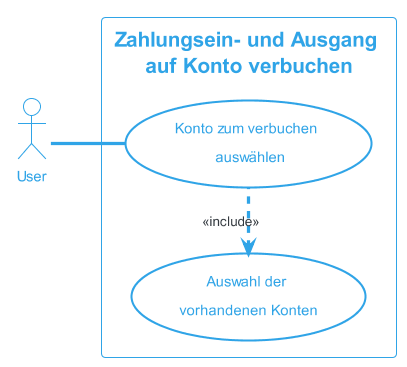
\includegraphics[width=0.5\linewidth]{content/diagrams/out/usecase/verbuchenAufKonto/ZahlungseingangaufKontoverbuchen.png}
    \caption{UC-Zahlungseingang auf Konto verbuchen}
    \label{ZahlungaufKonto}
  \end{center}
\end{figure}

\begin{table}[H]
  \newcolumntype{a}{>{\columncolor[HTML]{4473C5}}L}
  \centering
  \settowidth\tymin{\textbf{Kurzbeschreibung}}
  \setlength\extrarowheight{2pt}
  \begin{tabulary}{1.0\textwidth}{|a|m{14cm}|}
    \hline
    \textbf{Name}& Zahlungsein- und Ausgang auf Konto verbuchen\\
    \hline
    \textbf{Akteur}& Mitarbeiter:in der Liegenschaftsverwaltung\\
    \hline 
    \textbf{Beschreibung} & Bei einem Zahlungseingang, muss dieser auf ein entsprechendes Konto verbucht werden. Normalerweise gibt es aufgrund einer gestellten Rechnung einen Zahlungseingang. Wenn die Rechnung als bezahlt markiert wird, wird der Zahlungseingang auf das mit der Rechnung verknüpfte Konto verbucht \newline
    Falls es einen Zahlungsein- oder Ausgang gibt der nicht aufgrund einer Rechnung geschieht, muss dieser Eintrag manuell für das entsprechende Konto erstellt werden\\
    \hline
    \textbf{Daten} & Rechnungsnummer oder Zahlungsbetrag und Konto\\
    \hline
    \textbf{Auslöser} & Zahlungseingang\\
    \hline
    \textbf{Antwort} & Bestätigung, dass der Zahlungseingang verbucht wurde\\
    \hline
    \textbf{Kommentare} & Wenn das Konto zu dem der Zahlungsein- oder Ausgang erfasst werden soll noch nicht besteht, muss dies noch erstellt werden. Siehe \hyperref[kontoErstellen]{Konto erstellen \fref{kontoErstellen}}\\
    \hline
  \end{tabulary}
  \caption{UC-Zahlungsein- und Ausgang auf Konto verbuchen}
\end{table}

\newpage
\begin{figure}[H]
  \begin{center}
    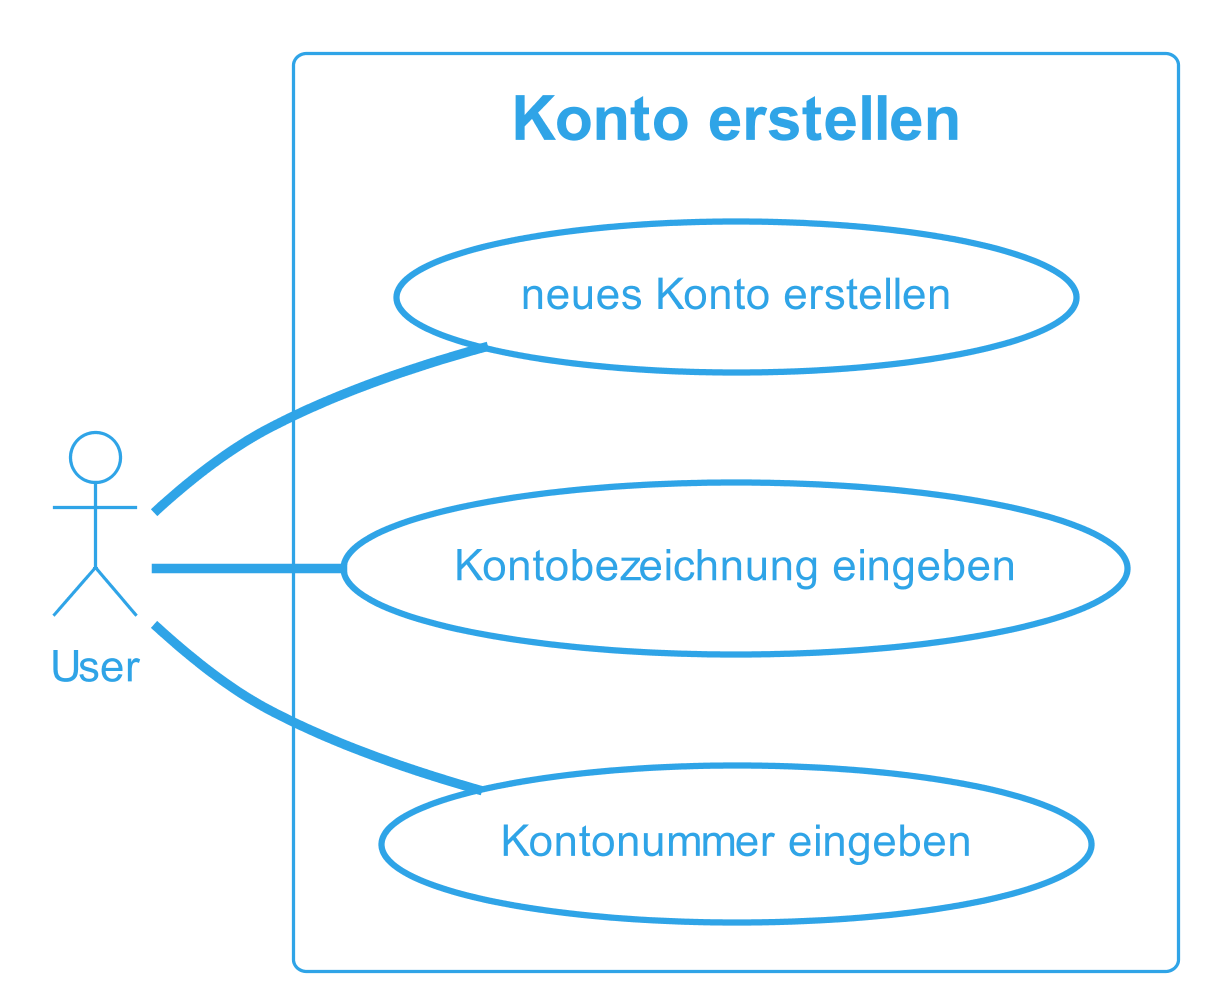
\includegraphics[width=0.5\linewidth]{content/diagrams/out/usecase/kontoErstellen/kontoErstellen.png}
    \caption{UC-Konto erstellen}
    \label{kontoErstellen}
  \end{center}
\end{figure}

\begin{table}[H]
  \newcolumntype{a}{>{\columncolor[HTML]{4473C5}}L}
  \centering
  \settowidth\tymin{\textbf{Kurzbeschreibung}}
  \setlength\extrarowheight{2pt}
  \begin{tabulary}{1.0\textwidth}{|a|m{14cm}|}
    \hline
    \textbf{Name}& Konto erstellen\\
    \hline
    \textbf{Akteur}& Mitarbeiter:in der Liegenschaftsverwaltung\\
    \hline 
    \textbf{Beschreibung} & Ein neues Konto zum verbuchen Der Zahlungen muss erstellt werden\\
    \hline
    \textbf{Daten} & Kontobezeichnung und Kontonummer\\
    \hline
    \textbf{Auslöser} & Benutzerbefehl, der von dem entsprechenden Akteur initiiert wird\\
    \hline
    \textbf{Antwort} & Bestätigung, dass das Konto erfolgreich erstellt wurde\\
    \hline
    \textbf{Kommentare} & -\\
    \hline
  \end{tabulary}
  \caption{UC-Konto erstellen}
\end{table}

\begin{figure}[H]
  \begin{center}
    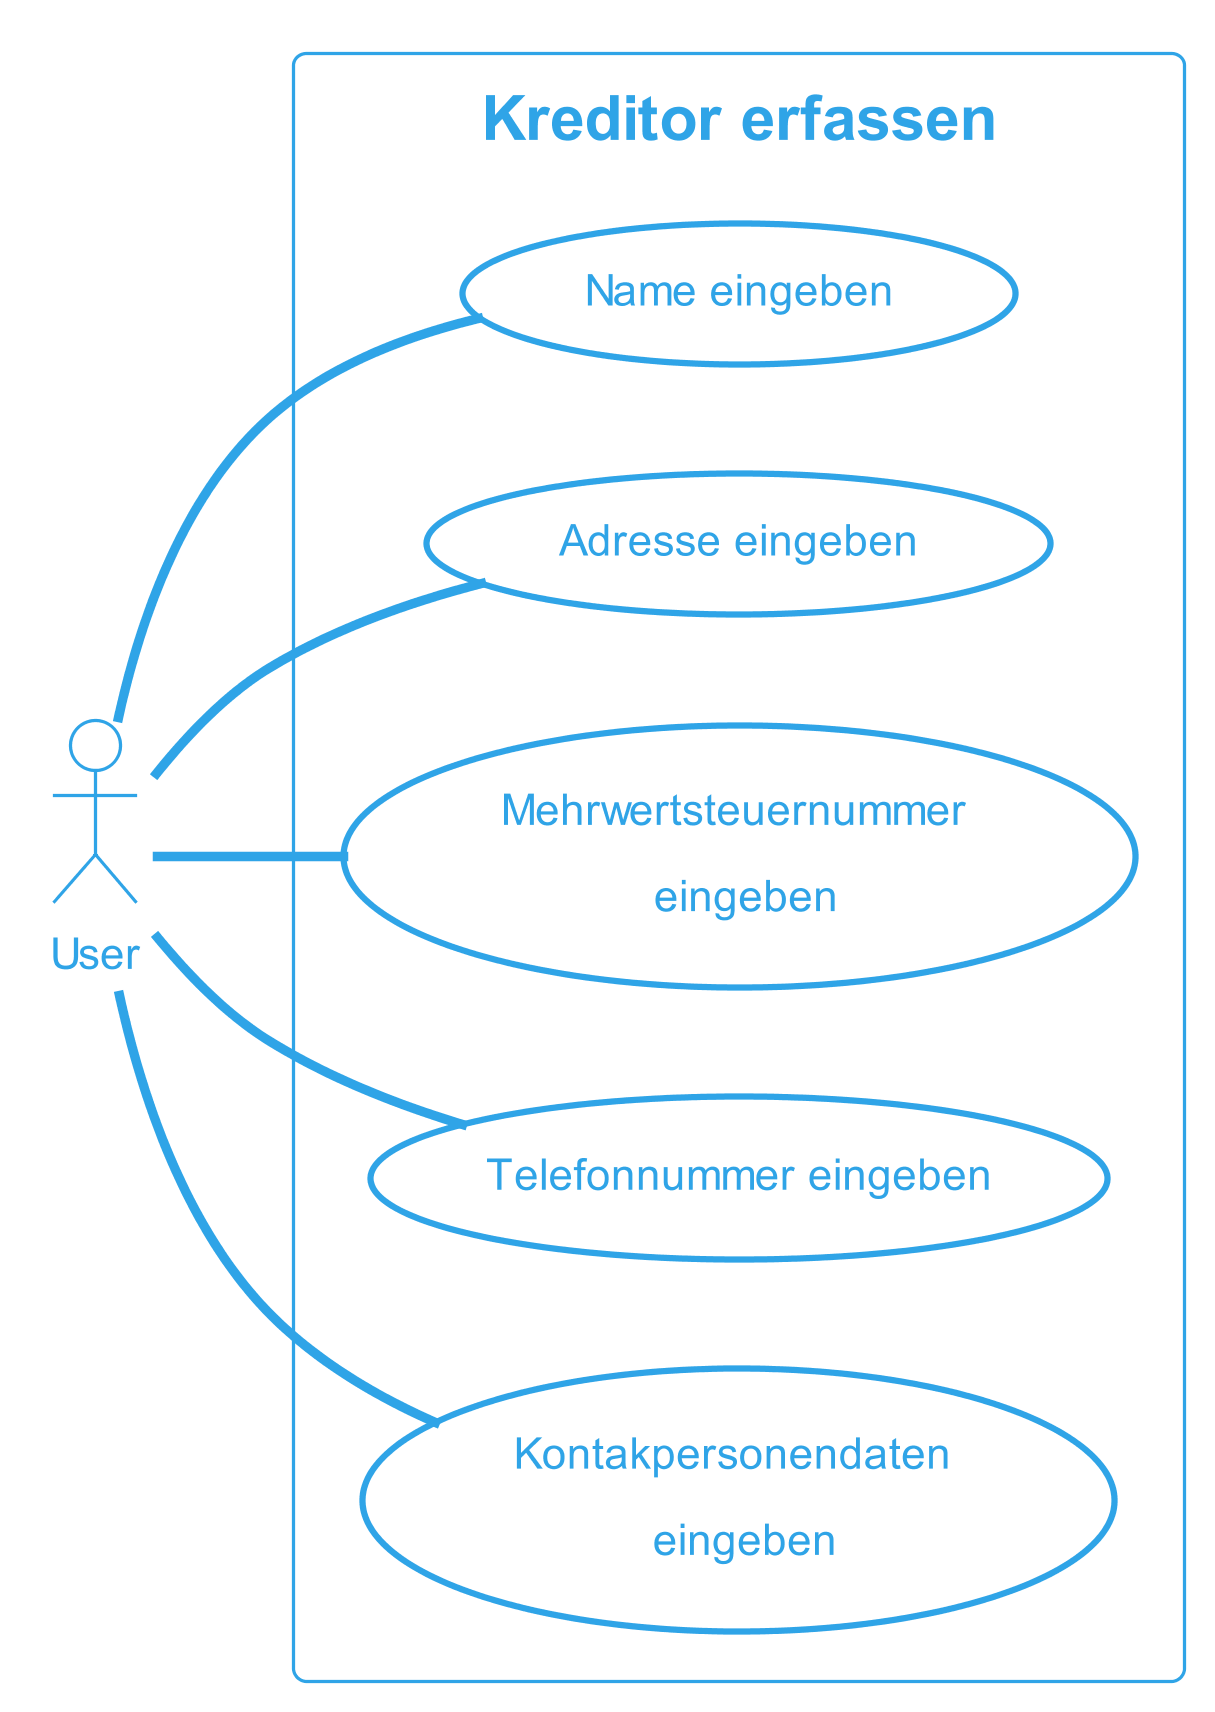
\includegraphics[width=0.5\linewidth]{content/diagrams/out/usecase/kreditorErfassen/Kreditor erfassen.png}
    \caption{UC-Kreditor erfassen}
    \label{kreditorErfassen}
  \end{center}
\end{figure}

\begin{table}[H]
  \newcolumntype{a}{>{\columncolor[HTML]{4473C5}}L}
  \centering
  \settowidth\tymin{\textbf{Kurzbeschreibung}}
  \setlength\extrarowheight{2pt}
  \begin{tabulary}{1.0\textwidth}{|a|m{14cm}|}
    \hline
    \textbf{Name}& Kreditor erfassen\\
    \hline
    \textbf{Akteur}& Mitarbeiter:in der Liegenschaftsverwaltung\\
    \hline 
    \textbf{Beschreibung} & Wir für einen Kreditor eine Rechnung erstellt der noch nicht erfasst wurde, wird dies hier gemacht\\
    \hline
    \textbf{Daten} & Vollständige Daten zum Kreditor\\
    \hline
    \textbf{Auslöser} & Benutzerbefehl der von dem entsprechenden Akteur initiiert wird\\
    \hline
    \textbf{Antwort} & Bestätigung, dass der Kreditor erfolgreich erfasst wurde\\
    \hline
    \textbf{Kommentare} & Normalwerkweise ist der Benutzer in der Applikation schon eingeloggt, weil erst beim erstellen der Rechnung bemerkt wird, dass der Kreditor noch nicht erfasst wurde. Für Miet-und Nebenkostenabrechnungen sind die Mieter die Kreditoren \\
    \hline
  \end{tabulary}
  \caption{UC-Kreditor erfassen}
\end{table}


\subsection{Sequenzdiagramme}

\subsection{Modellierung der Klassen}

\subsubsection{Klassendiagramm}
\begin{figure}[H]
  \begin{center}
    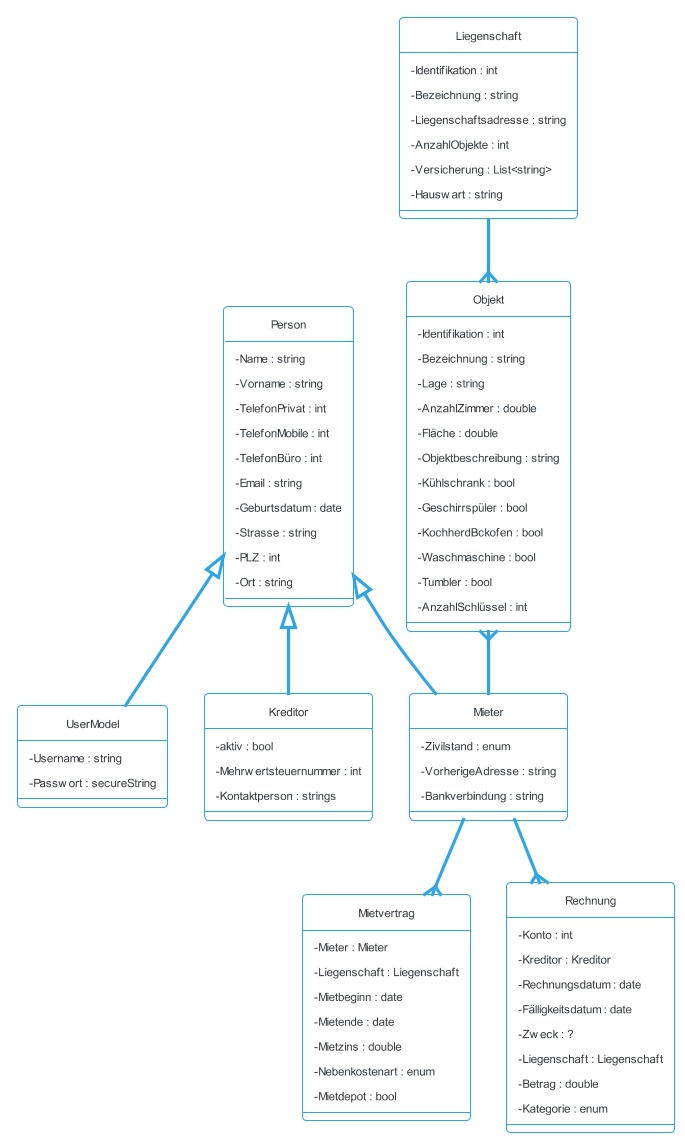
\includegraphics[width=0.8\linewidth]{content/diagrams/out/classdiagramm/ImmoGlobal.png}
    \caption{Klassendiagramm}
    \label{classdiagramm}
  \end{center}
\end{figure}

\subsubsection{Beschreibung der Fachklassen}

\subsection{Zustandsdiagramme}

\subsection{Modellierung der Datenbank}

\subsubsection{ERD}

\subsubsection{Beschreibung der Fachentitäten, Beziehungen und der referenziellen Integritätsbedingungen}

\subsection{Systemarchitektur}
Die Programmiersprache für die Applikation ist C\# mit dem aktuellen .net Core 6 Framework. Das GUI wird mit WPF aufgebaut und die gesamte Struktur im MVVM-Pattern gehalten. Um das GUI ansprechend zu gestalten, wird das NuGet-Paket ''Material-Design'' verwendet.\\
Für das persistieren der Daten wird das Entity-Framework verwendet, mit welchem bereits in einem früheren Projekt Erfahrung gesammelt werden konnte.
\subsection{Testkonzept} \label{testkonzept}
\subsubsection{Vorgehen}
\subsubsection{Testobjekte}
\subsubsection{Testfälle}
\subsection{Einführungskonzept}
\subsection{GUI-Design}